\section{Appendix: Spectral clustering and other methods}
\subsection*{}

\textbf{Spectral Partitioning} 
\cite{von2007tutorial, naumov2016parallel, WikipediaGraphPartition, WikipediaSpectralClustering},
is a common technique for partitioning graphs. The idea is to construct a
Laplacian type matrix \cite{WikipediaLaplacianMatrix} for the graph
$G$,
analyze its eigenvalues and eigenvectors and construct a $2$-partition of $G$.
It is possible to create a hierarchical partitioning of $G$ by repeating the
process on each subdivision.

The problem of finding the best graph partition, also called the minimal cut
problem is NP-hard. Spectral partitioning methods are heuristics that
approximate the solution in 'real life' classes of networks.

\subsection*{}

\begin{mydef}
\label{def:Laplacian}
Let $G$ be a bidirectional graph with adjacency matrix $A$ and diagonal degree
matrix $D$.
Then the following matrices are its \textbf{graph Laplacian}, and its
\textbf{symmetric\textemdash
, row\textendash normalized\textemdash and column\textendash normalized\textemdash Laplacians}:  

\begin{equation}
\begin{aligned}
L & = D - A \\
L_s & = D^{-1/2}LD^{-1/2} = I - D^{-1/2}AD^{-1/2} \\
L_r & = D^{-1}L = I - D^{-1}A \\
L_c & = LD^{-1} = I - AD^{-1}
\end{aligned}
\end{equation}
\end{mydef}

Consider the connected graph $G$ and its adjacency matrix $A$. We create the transition
matrix by normalizing it: $T = AD^-1$, and finally we choose a restart parameter
$\alpha$ and create the diffusion matrix $K = \alpha[I - (1 -
\alpha) T]^{-1}$. Theorem
\ref{thm:AKTcharacteristics} assures us that $K$ and $T$ have the same
eigenvectors and the orders of their corresponding eigenvalues are the same. The
eigenvalues are all real and therefore the eigenvectors are real as well. And
the eigenvalues of $K$ are all non-negative.

The matrix $K^{-1} = \alpha^{-1} [I - (1- \alpha) T]$ is closely related to the
symmetric Laplacian $L_s$ and thecolumn-normalized Laplacian $L_c$. The added parameter $0 \lt \alpha \lt 1$
neither changes the eigenvectors, nor the order of the corresponding eigenvalues.

The smallest eigenvalue ,$0$ of $L$ and $L_s$
corresponds to the largest eigenvalue $1$ of and $T$ and its eigenvector is
(can be chosen as) all positive. 
Any other eigenvector of $L$ (which corresponds to an eigenvector of $T$) must
contain both positive and negative components due to \ref{thm:perron1}.

It's the eigenvector of the second smallest
eigenvalue $L$ or $L_s$ which is commonly used in 
They are commonly referred to as the \textbf{Fiedler} eigen-pair in the literature.
for spectral partitioning \cite{naumov2016parallel}. The simplest method is to
use the sign of the components of
eigenvector of the second smallest eigenvalue of $L$ or $L_s$.
This eigen-pair corresponds to the second largest eigenvalue of $T$

In \textcite{newman2006modularity} there is a particular type of spectral
partitioning which uses a matrix which the author called the modularity matrix.
It has the advantage over the Laplacian in that its greatest eigenvalue may be
positive or negative which is used to indicate or suggest the existence of
community structure in the graph. However the normalized Laplacians $L_r$ and
$L_c$ are more natural in the context of the random walk or propagation method
and recommended for example in \cite{von2007tutorial}.


\begin{figure}
\begin{framed}
\centering
\begin{subfigure}[b]{0.5\textwidth}
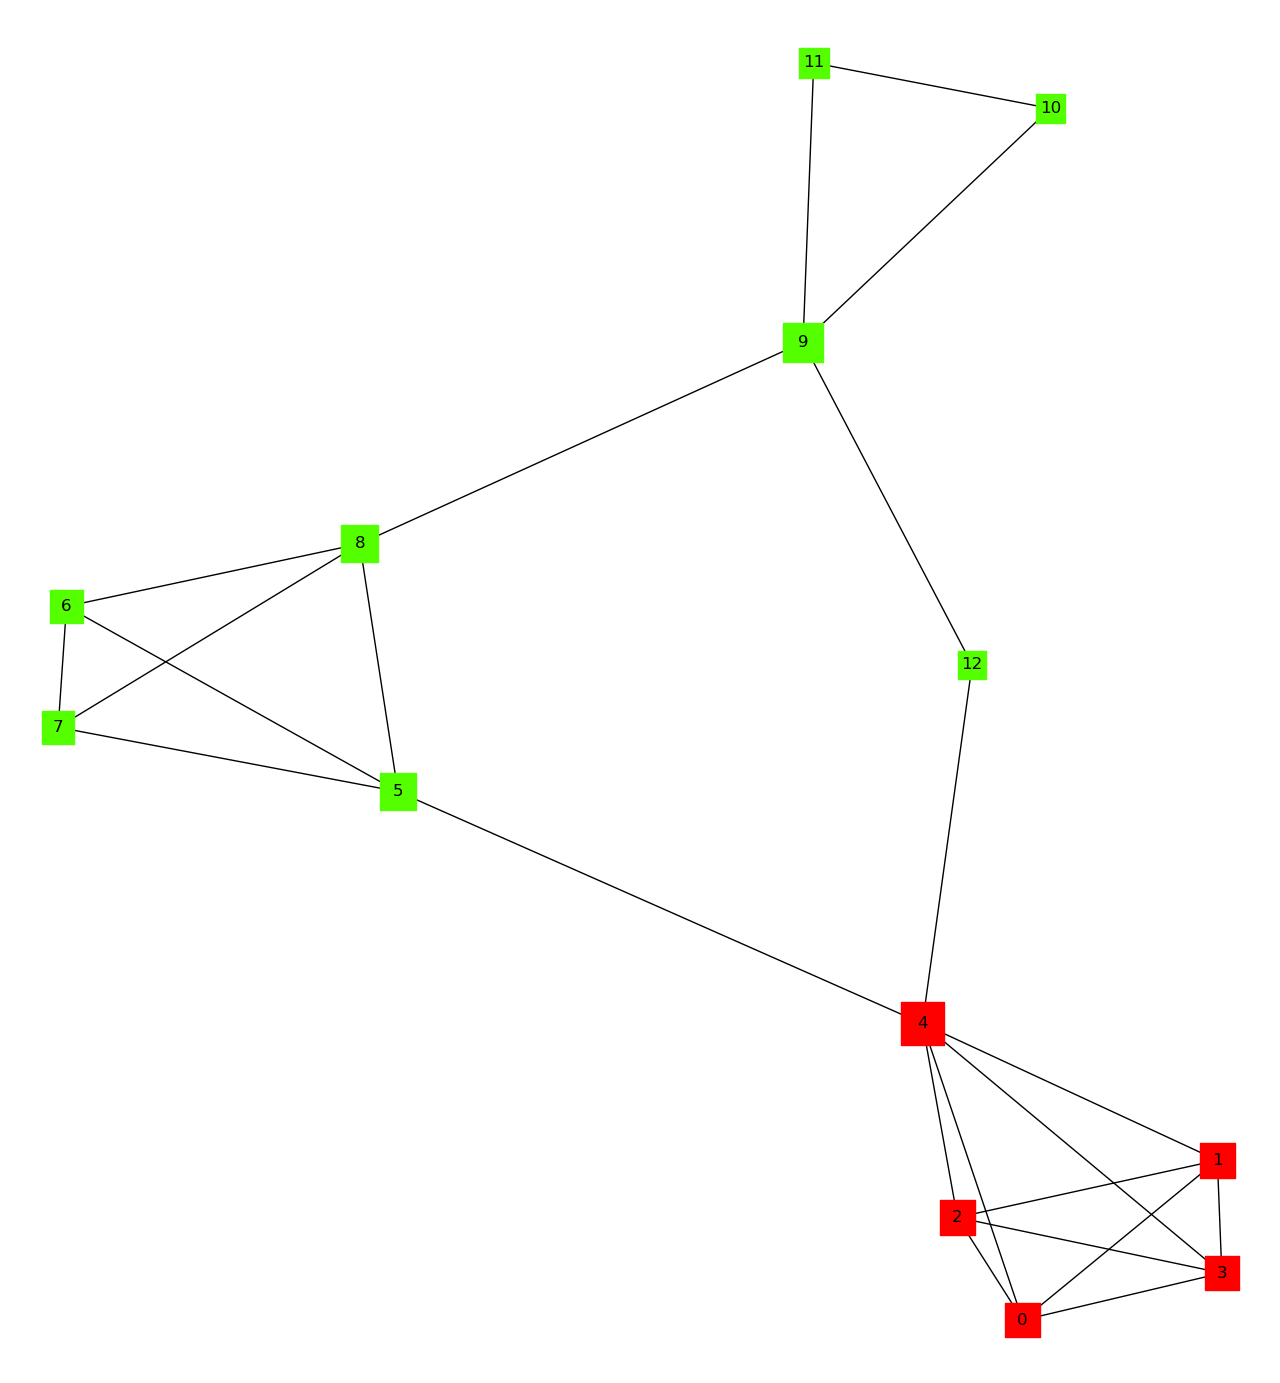
\includegraphics[width=\textwidth]{figures/example_spectralT2clustering.png}
\caption{A spectral clustering using the sign of the Fiedler eigenvector.}
\label{fig:toygraphspectralclustering}
\end{subfigure}
%add desired spacing between images, e. g. ~, \quad, \qquad, \hfill etc. 
%(or a blank line to force the subfigure onto a new line)
\begin{subfigure}[b]{0.5\textwidth}
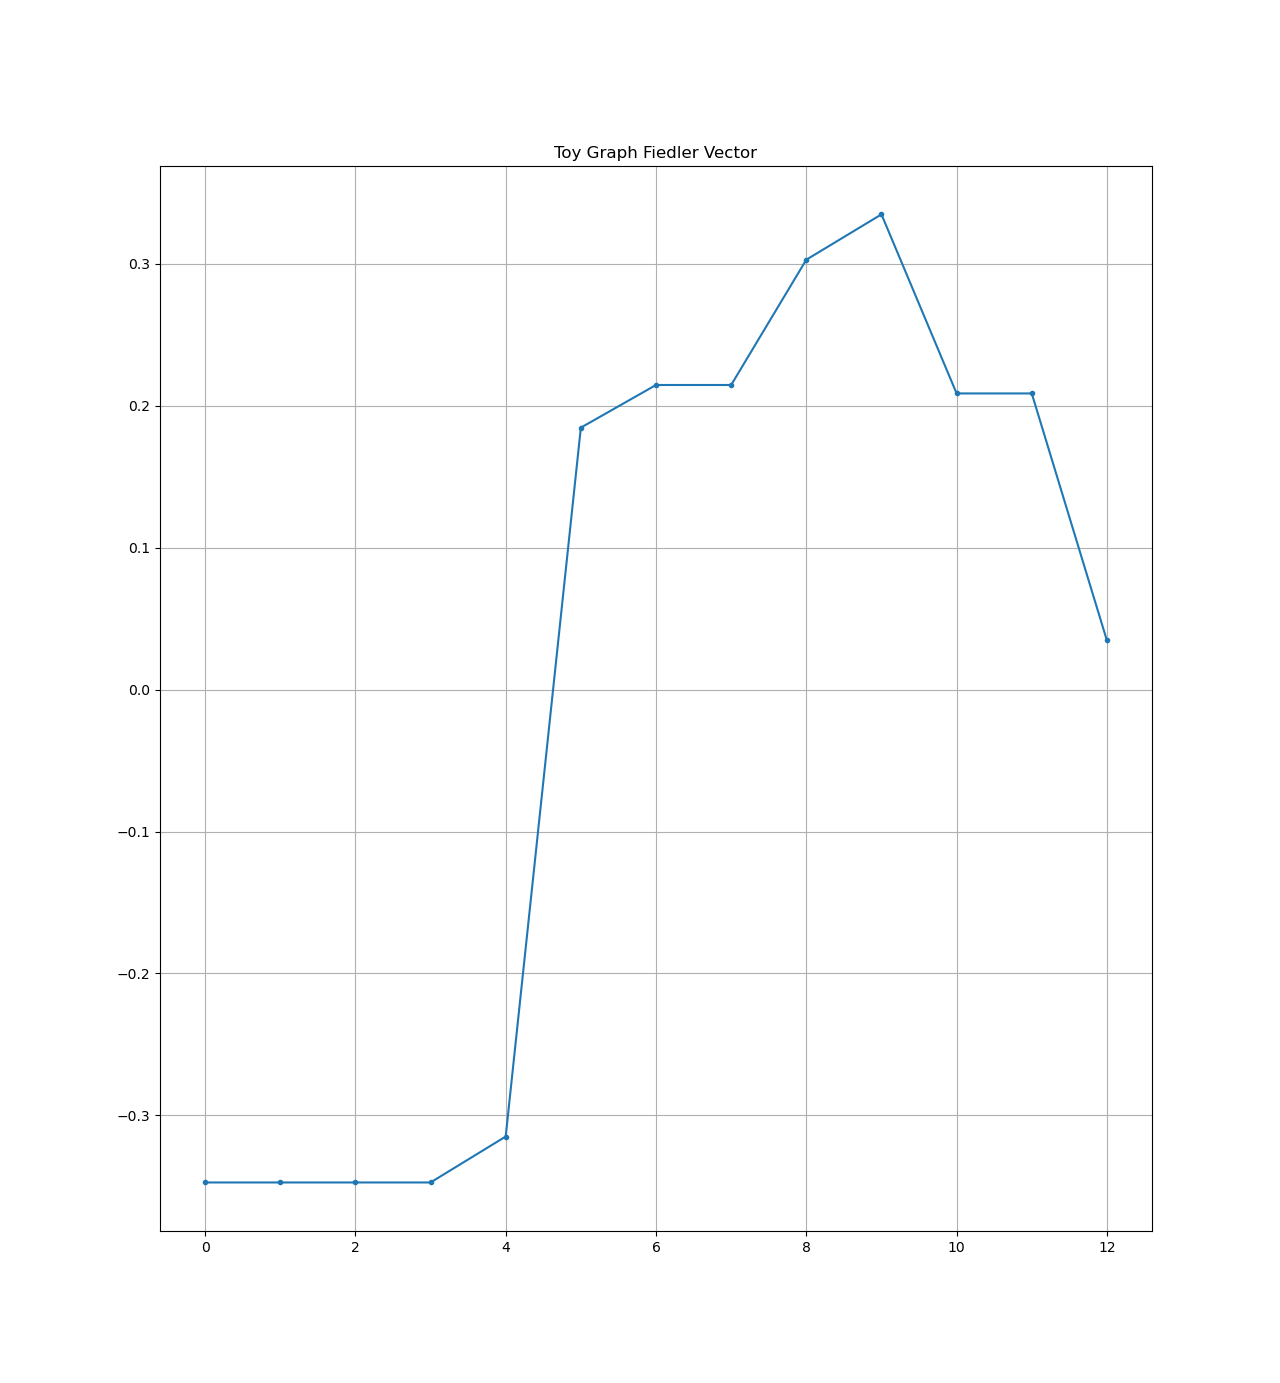
\includegraphics[width=\textwidth]{figures/Toygraph_Fiedler.png}
\caption{Plot of the Fiedler vector's components, showing a clear subdivision
between the positive and the negative components.}
\label{fig:toygraphfiedlerplot}
\end{subfigure}
%add desired spacing between images, e. g. ~, \quad, \qquad, \hfill etc. 
%(or a blank line to force the subfigure onto a new line)
\caption{}
%\label{fig:exampleCoolWarmClustering}
\end{framed}
\end{figure}

\begin{figure}
\begin{framed}
\centering
\begin{subfigure}[b]{0.5\textwidth}
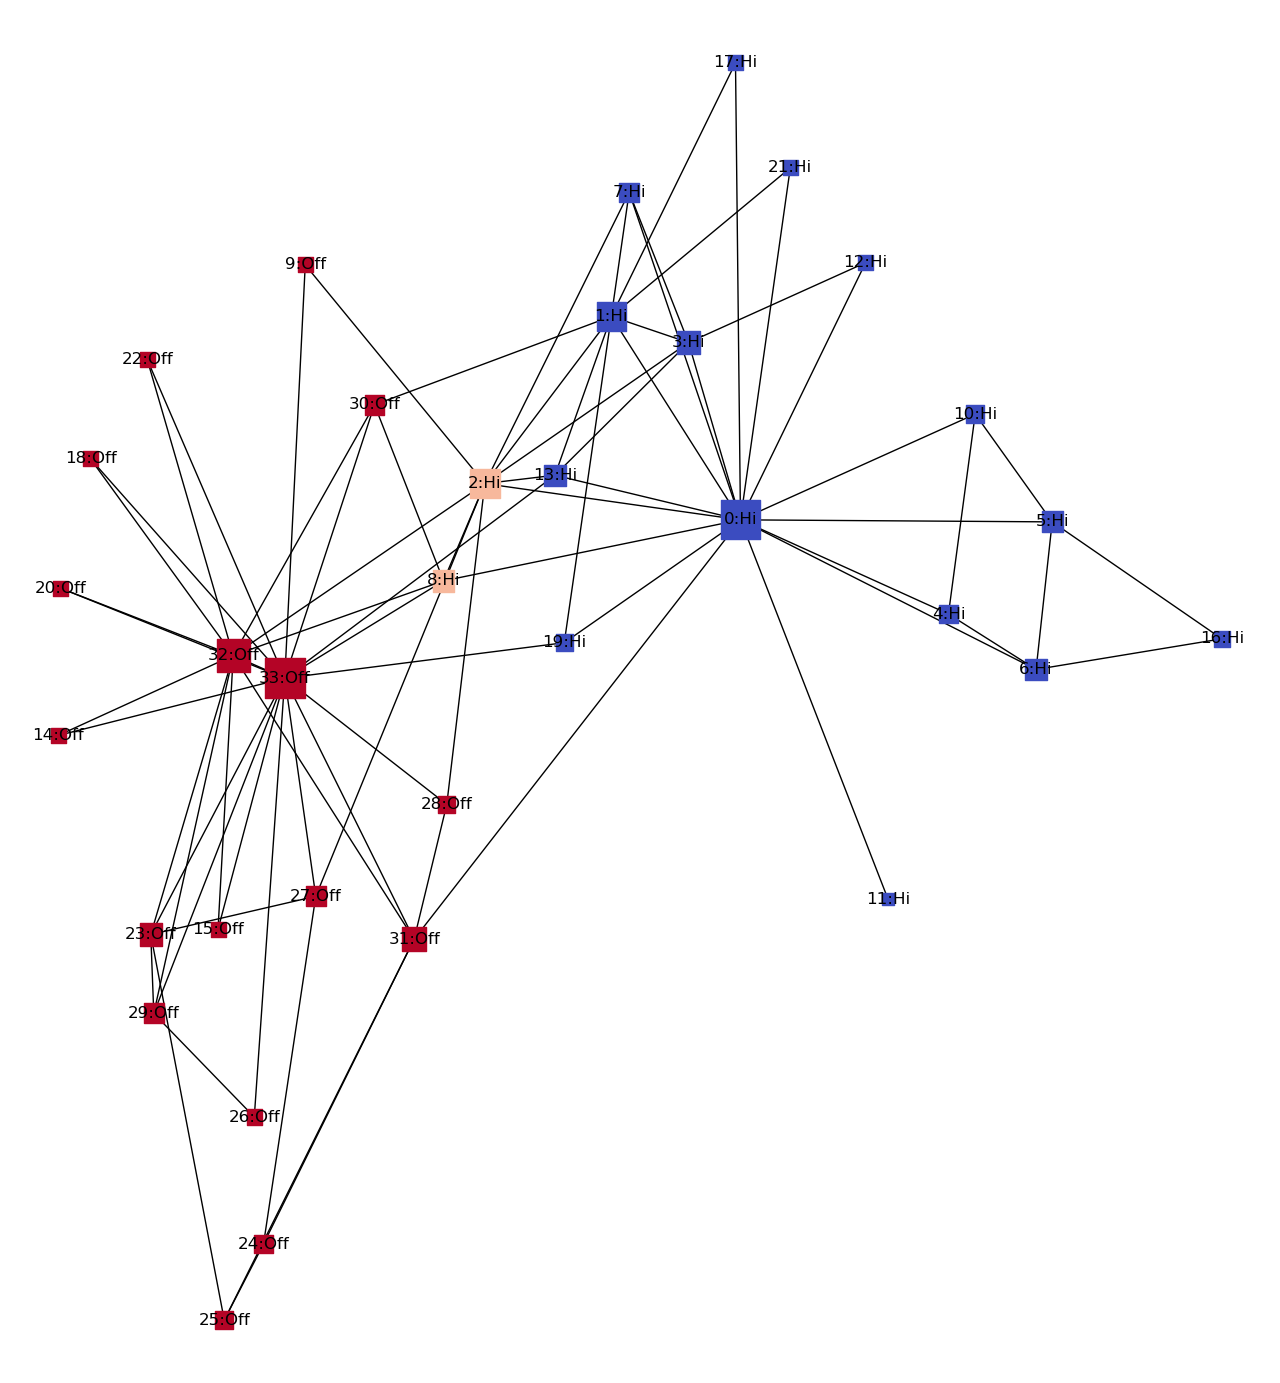
\includegraphics[width=\textwidth]{figures/Karate_spectralT2clustering.png}
\caption{Spectral clustering of the Karate Club network using the Fiedler
eigenvector signs. There are $2$ deviations from the actual partition, both are
borderline nodes which are harder to resolve. The $8$ node mistake is in common
with the naive algorithm of the previous section.}
\label{fig:karatespectral}
\end{subfigure}
%add desired spacing between images, e. g. ~, \quad, \qquad, \hfill etc. 
%(or a blank line to force the subfigure onto a new line)
\begin{subfigure}[b]{0.5\textwidth}
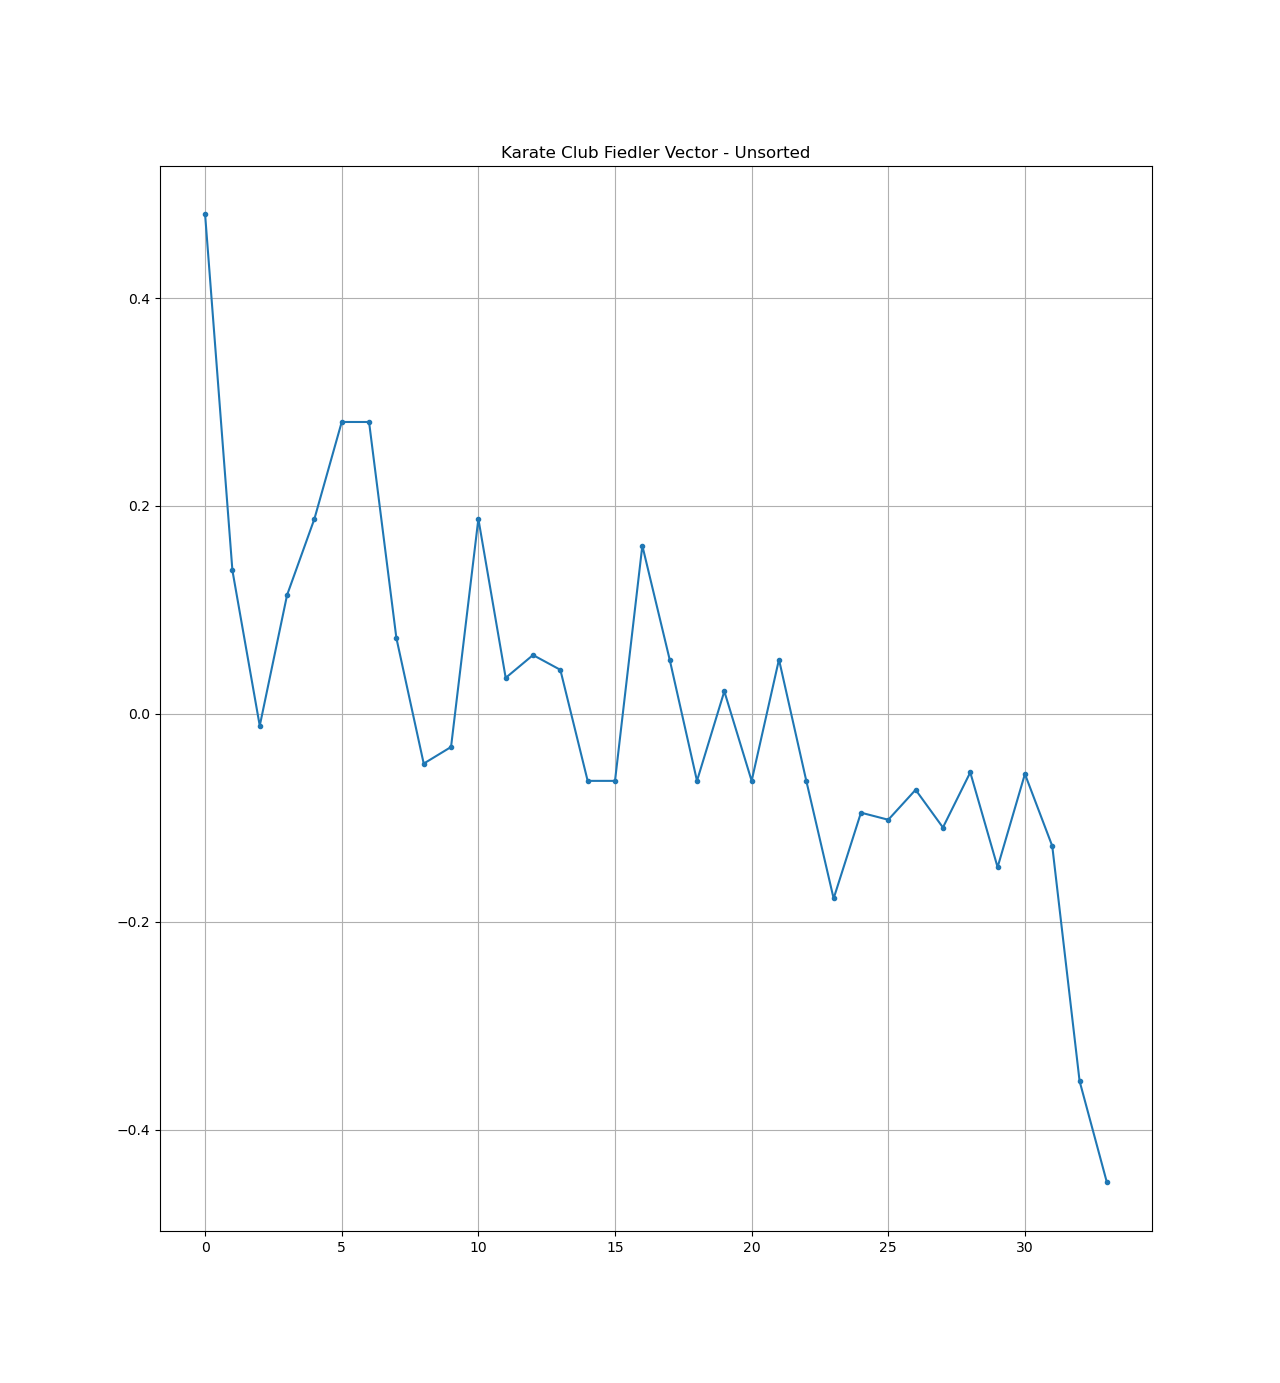
\includegraphics[width=\textwidth]{figures/karate_fiedler_unsorted.png}
\caption{Plot of the Fiedler Vector of the Karate Club. The split between
negative and positive values is much less dramatic but nonetheless still visible.}
\label{fig:karatefiedlerplot}
\end{subfigure}
%add desired spacing between images, e. g. ~, \quad, \qquad, \hfill etc. 
%(or a blank line to force the subfigure onto a new line)
%\caption{}
%\label{fig:exampleCoolWarmClustering}
\end{framed}
\end{figure}

